% Resume of João Gabriel Salvador Paiva — general software development profile
% Single-column layout, fully selectable text, no tables or text boxes (ATS-friendly).
\documentclass[10.5pt,a4paper]{article}

\usepackage[T1]{fontenc}
\usepackage[utf8]{inputenc}
\usepackage[english]{babel}
\usepackage{lmodern}
\usepackage[margin=1.5cm,top=1.2cm,bottom=1.2cm]{geometry}
\usepackage{graphicx}
\usepackage{enumitem}
\usepackage{titlesec}
\usepackage{xcolor}
\usepackage[hidelinks]{hyperref}
\usepackage{microtype}
\usepackage{needspace}

\definecolor{azul}{HTML}{14375A}

\hypersetup{
  pdftitle={Joao Gabriel Salvador Paiva - Software Developer},
  pdfauthor={Joao Gabriel Salvador Paiva},
  pdfsubject={Resume - Software Developer},
  pdfkeywords={Python, Dart, Django, FastAPI, REST APIs, microservices, Flutter, PostgreSQL, Redis,
  RabbitMQ, Docker, AWS, GitHub Actions, CI/CD, PyTest, Clean Code, SOLID, Scrum, LLMs}
}

\pagestyle{empty}
\setlength{\parindent}{0pt}
\setlength{\emergencystretch}{2em}
\setlist[itemize]{leftmargin=3.6mm,itemsep=1pt,topsep=2pt,parsep=0pt,label=\textbullet}

\titleformat{\section}{\bfseries\large\color{azul}}{}{0em}{}[\vspace{-1.2ex}\rule{\linewidth}{0.6pt}]
\titlespacing{\section}{0pt}{2.2ex}{1.2ex}

\newcommand{\cargo}[4]{%
  \Needspace*{5\baselineskip}%
  \textbf{#1} \textnormal{---} #2 \hfill \textnormal{#3}\\
  \textit{\small #4}\vspace{0.4ex}
}

\begin{document}

%% ---------- Header ----------
\begin{minipage}[c]{0.78\textwidth}
\raggedright
{\LARGE\bfseries\color{azul} João Gabriel Salvador Paiva}\\[0.6ex]
{\large Software Developer}\\[0.9ex]
\small
Campina Grande, Brazil (open to remote work)\\
\href{mailto:joaogabrielsalvadorpaiva@gmail.com}{joaogabrielsalvadorpaiva@gmail.com} $\cdot$ +55 (83) 98863-6734\\
\href{https://github.com/Ilusinusmate}{github.com/Ilusinusmate} $\cdot$
\href{https://www.linkedin.com/in/jo\%C3\%A3o-gabriel-salvador-paiva-805283286/}{linkedin.com/in/joão-gabriel-salvador-paiva} $\cdot$
\href{https://ilusinusmate.github.io/Ilusinusmate/}{ilusinusmate.github.io/Ilusinusmate}
\end{minipage}\hfill
\begin{minipage}[c]{0.2\textwidth}
\raggedleft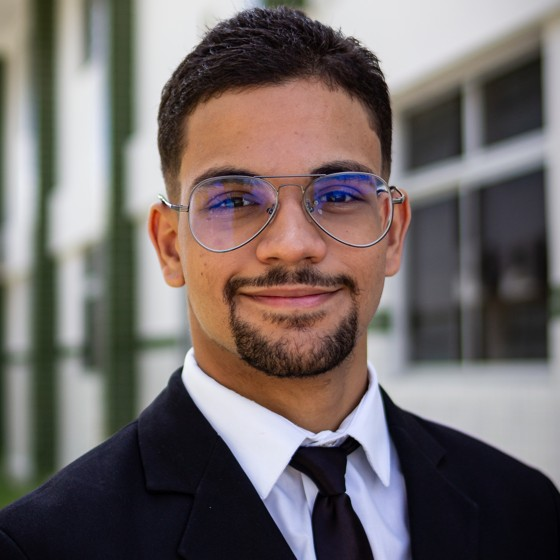
\includegraphics[width=2.7cm]{foto.jpg}
\end{minipage}

%% ---------- Summary ----------
\section*{Summary}
Software developer with experience in \textbf{Python backend} and \textbf{Flutter/Dart mobile
development}, building \textbf{REST APIs}, microservices and production applications. At Logon, I
am responsible for the \textbf{Central da Escola} app, with more than \textbf{50 thousand active
users}, and for Python/FastAPI supporting services, while also handling testing, CI/CD and
publication on Android and iOS stores. I also built an ERP, POS and e-commerce SaaS with
Django/Python and PostgreSQL, and conduct research on AI, LLMs and Software Engineering. Computer
Science undergraduate at UFCG and ICT resident at VIRTUS-CC/UFCG.

%% ---------- Technical Skills ----------
\section*{Technical Skills}
\textbf{Languages:} Python, Dart, JavaScript, TypeScript, SQL, C\\
\textbf{Backend:} Django, Django REST Framework, FastAPI, REST APIs, microservices, authentication,
integrations between systems\\
\textbf{Mobile:} Flutter, Dart, Android, iOS, store publication, BLoC, WebSocket, componentization\\
\textbf{Data:} PostgreSQL, NoSQL databases, Redis, MinIO, data modeling\\
\textbf{Infrastructure and DevOps:} RabbitMQ, Docker, AWS (S3, CloudFront), Railway, Render, Nginx,
Linux, GitHub Actions, CI/CD, OpenTelemetry, Grafana, logging\\
\textbf{Quality:} PyTest, mocks, automated testing, code review\\
\textbf{Engineering:} Clean Code, SOLID, DRY, DDD, design patterns, technical documentation,
Scrum/Kanban, distributed systems

%% ---------- Professional Experience ----------
\section*{Professional Experience}

\cargo{Logon Informática}{Mobile \& Backend Developer}{Jan 2025 -- Present}{Software house for
education management, public administration and other sectors}
\begin{itemize}
  \item Develop Python/FastAPI microservices, REST APIs, asynchronous communication with
        \textbf{RabbitMQ} and object storage with \textbf{MinIO} for the Central da Escola app.
  \item Sole developer of the application since \textbf{version 3}, using \textbf{Flutter/Dart},
        with more than \textbf{50 thousand active users} on Android and iOS.
  \item Lead the mobile area and handle development, testing, \textbf{CI/CD}, store publication,
        logging, documentation and liaison with internal teams and third-party systems.
\end{itemize}

\cargo{Empório Sertanejo}{Full-stack Developer --- technical lead}{Dec 2023 -- Sep 2025}{Retail
franchise; proprietary ERP, POS and e-commerce SaaS}
\begin{itemize}
  \item \textbf{Led 3 developers} in building a SaaS that unified \textbf{ERP, POS and e-commerce},
        using \textbf{Django/Python}, \textbf{PostgreSQL} and \textbf{Docker}.
  \item Implemented automated tests with PyTest and mocks, CI/CD with GitHub Actions and
        observability with OpenTelemetry and Grafana.
  \item Conducted requirements gathering and client negotiation, delivering loyalty programs,
        coupons, notifications and online sales.
\end{itemize}

\cargo{VIRTUS-CC / Softex (UFCG)}{ICT Resident --- ISE group researcher}{Nov 2025 --
Present}{One-year software residency program: 240h of training + practical immersion}
\begin{itemize}
  \item Ranked \textbf{1st} in the selection process (96/100 in the titles evaluation and 100/100
        in the interview).
  \item Training in Software Engineering, agile methodologies, IoT, machine learning and design
        thinking, with projects in a multidisciplinary squad.
  \item Research LLMs applied to Software Engineering in the \textbf{Intelligent Software
        Engineering} group, with an article accepted at \textbf{XP 2026} (Springer LNBIP).
\end{itemize}

\cargo{Animalesko}{Backend Developer (volunteer)}{Apr 2024 -- Sep 2024}{Social startup supporting
stray animals}
\begin{itemize}
  \item Designed the application's cross-platform backend architecture, prioritizing low resource
        consumption, and documented the technical decisions.
\end{itemize}

\cargo{IFPB (CNPq / LAPLIN)}{Scholarship researcher and Python instructor}{2023 -- 2024}{Natural
Language Analysis and Processing Laboratory}
\begin{itemize}
  \item Worked as a research scholarship holder, leading the student group in two projects, and
        taught \textbf{Python} classes to approximately 60 students.
  \item Conducted an experiment comparing programming learning with and without AI support, with
        publications at national events.
\end{itemize}

%% ---------- Projects ----------
\section*{Projects}
\begin{itemize}
  \item \textbf{pdfa-parser} --- open-source Python library published on PyPI for converting PDFs to
        PDF/A and automatically validating them with GhostScript and VeraPDF, with synchronous and
        asynchronous APIs, CLI and container execution:
        \href{https://pypi.org/project/pdfa-parser}{pypi.org/project/pdfa-parser}
  \item \textbf{Contratexto} --- multiplayer web game built with FastAPI, WebSocket and semantic
        similarity, using NLP and an asynchronous queue:
        \href{https://contratexto.onrender.com}{contratexto.onrender.com}
  \item \textbf{Central da Escola} --- Flutter school application with more than
        \textbf{50 thousand active users}, published on Android and iOS, with its own microservices.
  \item \textbf{TodoApp} --- Flutter application with Clean Code, SOLID, componentization, context
        isolation and BLoC, running on Android and Linux Desktop:
        \href{https://github.com/Ilusinusmate/todoApp}{github.com/Ilusinusmate/todoApp}
  \item \textbf{Corretor ONHB} --- application commissioned by IFPB teachers for automatic correction
        of National History Olympiad exams, built with Flutter and Electron.
\end{itemize}

%% ---------- Education ----------
\section*{Education}
\textbf{Bachelor of Computer Science} --- Federal University of Campina Grande (UFCG)
\hfill Jan 2025 -- 2030\\
\textbf{Integrated Technical Program} --- Federal Institute of Paraíba (IFPB)
\hfill Mar 2022 -- Dec 2024\\
\textbf{Additional training} --- Flutter Specialist and Python Backend Developer (DIO)

%% ---------- Publications and Awards ----------
\section*{Publications and Awards (selected)}
\begin{itemize}
  \item \textbf{8 scientific works} published on AI, LLMs and Software Engineering, including an
        article at \textbf{XP 2026} (Springer LNBIP, 2nd author) and articles at \textbf{WEI 2025}
        and \textbf{WICS 2024} (Brazilian Computer Society).
  \item \textbf{Best expanded abstract} in the Scientific and Technological Initiation --- ICT
        category at the \textbf{5th SIMPIF} (2023).
  \item \textbf{Champion of the Paraíba Informatics Olympiad} (2023), \textbf{gold} in the Advanced
        Junior category (2026) and finalist in the Brazilian Informatics Olympiad (2023).
\end{itemize}

\section*{Languages}
Portuguese (native) $\cdot$ English (advanced --- reading, writing and professional communication)
$\cdot$ Libras/Brazilian Sign Language (intermediate)

\end{document}
